\section{Experiment Set-up \& Extra Results}
\label{app:setup}
\subsection*{Experiment Set-up}
\begin{table}[htbp]
    \centering
    \caption{Hardware and Software Specifications.}
    \label{tab:system_specs}
    \begin{tabular}{ll}
        \toprule
        \textbf{Component} & \textbf{Specification} \\
        \midrule
        CPU & AMD Ryzen 7 5800X (@ 4.85 GHz) \\
        GPU & NVIDIA GeForce RTX 3080 Ti \\
        RAM & 32 GB \\
        OS & Ubuntu 24.10 (Kernel 6.11.0) \\
        Framework & FL-bench (based on PyTorch) \\
        \bottomrule
    \end{tabular}
\end{table}    
\label{subsec:setup}
\noindent\textbf{Implementation Details.} 
We implemented our proposed framework using the Python programming language and the FL-bench ecosystem\footnote{https://github.com/KarhouTam/FL-bench/tree/master}. The experiments were conducted on a high-performance workstation to ensure reproducibility. The detailed hardware and software specifications are listed in Table~\ref{tab:system_specs}.

\noindent\textbf{Hardware Environment.} 
The simulations were executed on a machine equipped with an AMD Ryzen 7 5800X CPU (8 cores, 16 threads, clocked at 4.85 GHz) and 32 GB of RAM. For model training and aggregation acceleration, we utilized a single NVIDIA GeForce RTX 3080 Ti GPU with 12 GB of VRAM.

\noindent\textbf{Software Environment.} 
The system runs on the Ubuntu 24.10 operating system (Kernel 6.11.0). All deep learning models were implemented using PyTorch within the FL-bench framework.


\subsection*{Multi-tier prototype representations}
\label{sec:tsne_analysis}
\begin{figure}
    \centering
    \begin{minipage}[c]{\textwidth}
        \centering
        % --- Hình T-SNE 1 (Bên trên) ---
        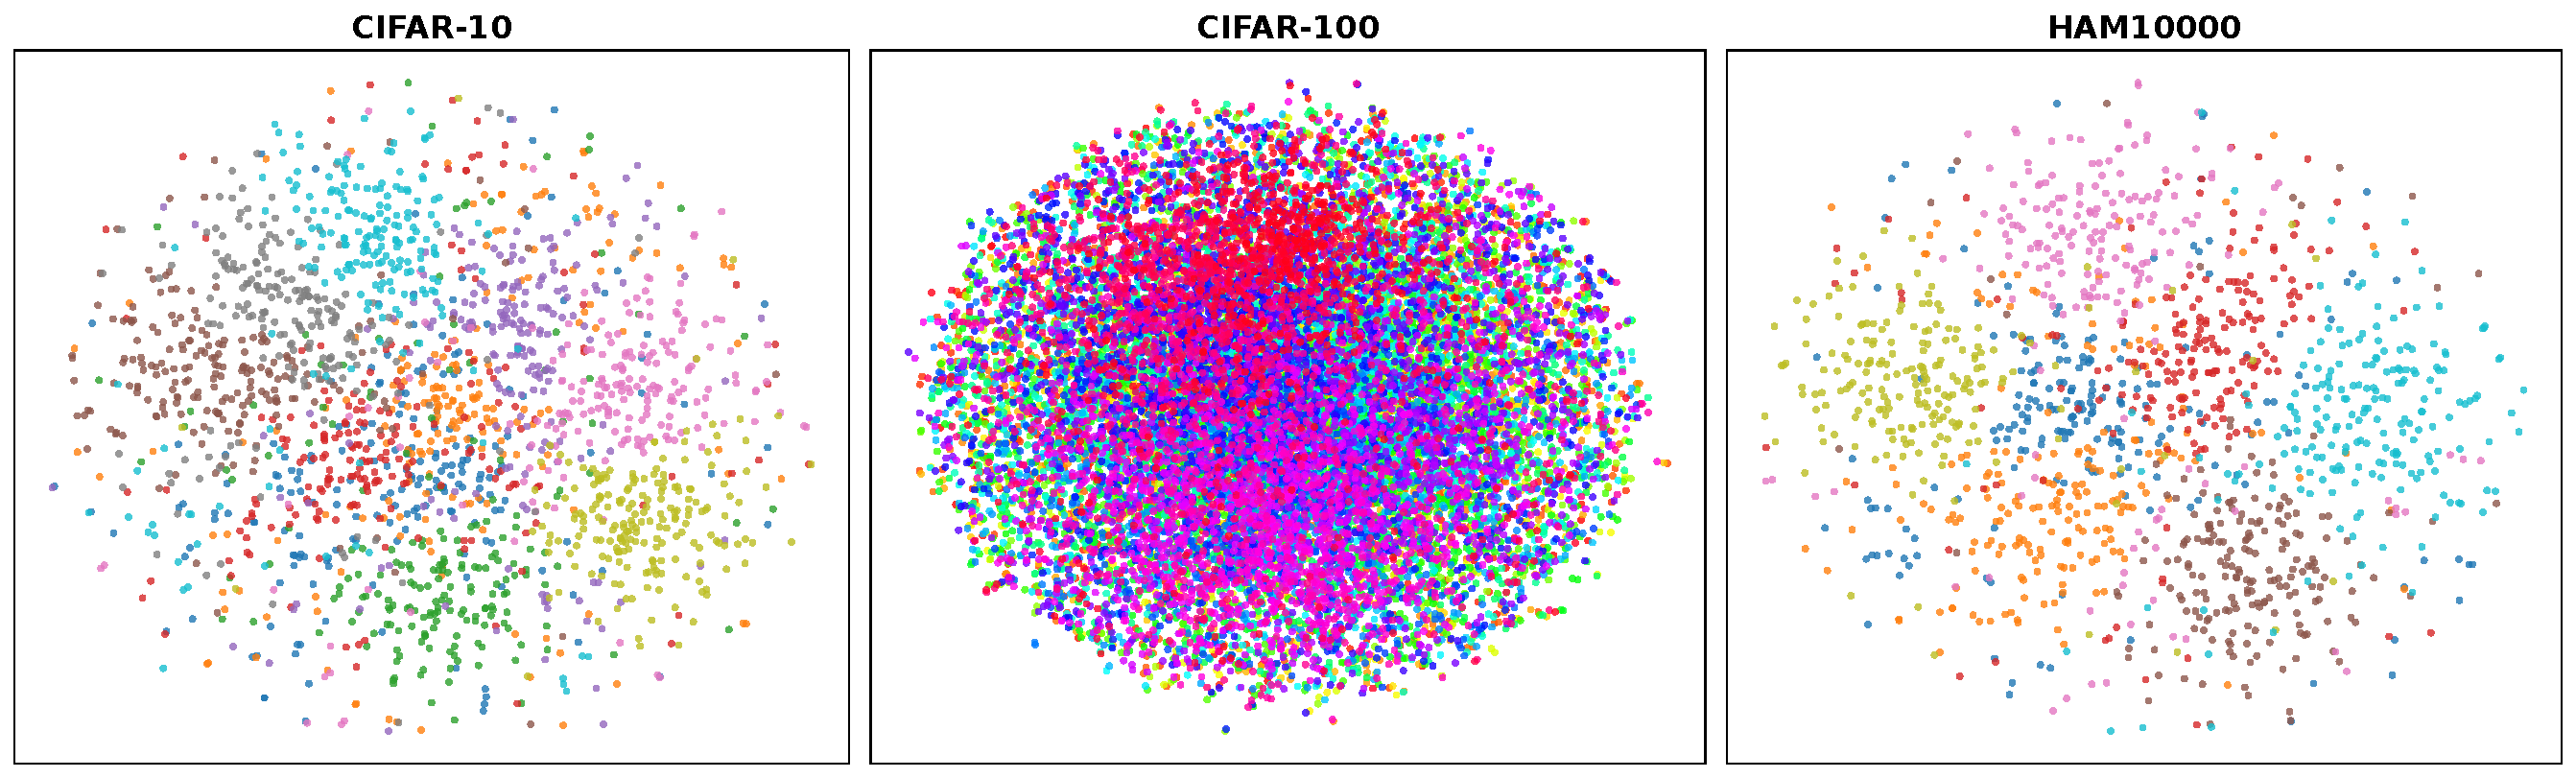
\includegraphics[width=\linewidth]{Figures/tsne_tier1_synthetic.pdf}
        \caption{Raw client features. Unaligned local training causes heavily overlapped representations before edge aggregation.}
        \label{fig:tsne_tier1}
        
        \vspace{1em} % Đã giảm khoảng cách từ 1.5em xuống 1em vì caption đã ngắn hơn
        
        % --- Hình T-SNE 2 (Bên dưới) ---
        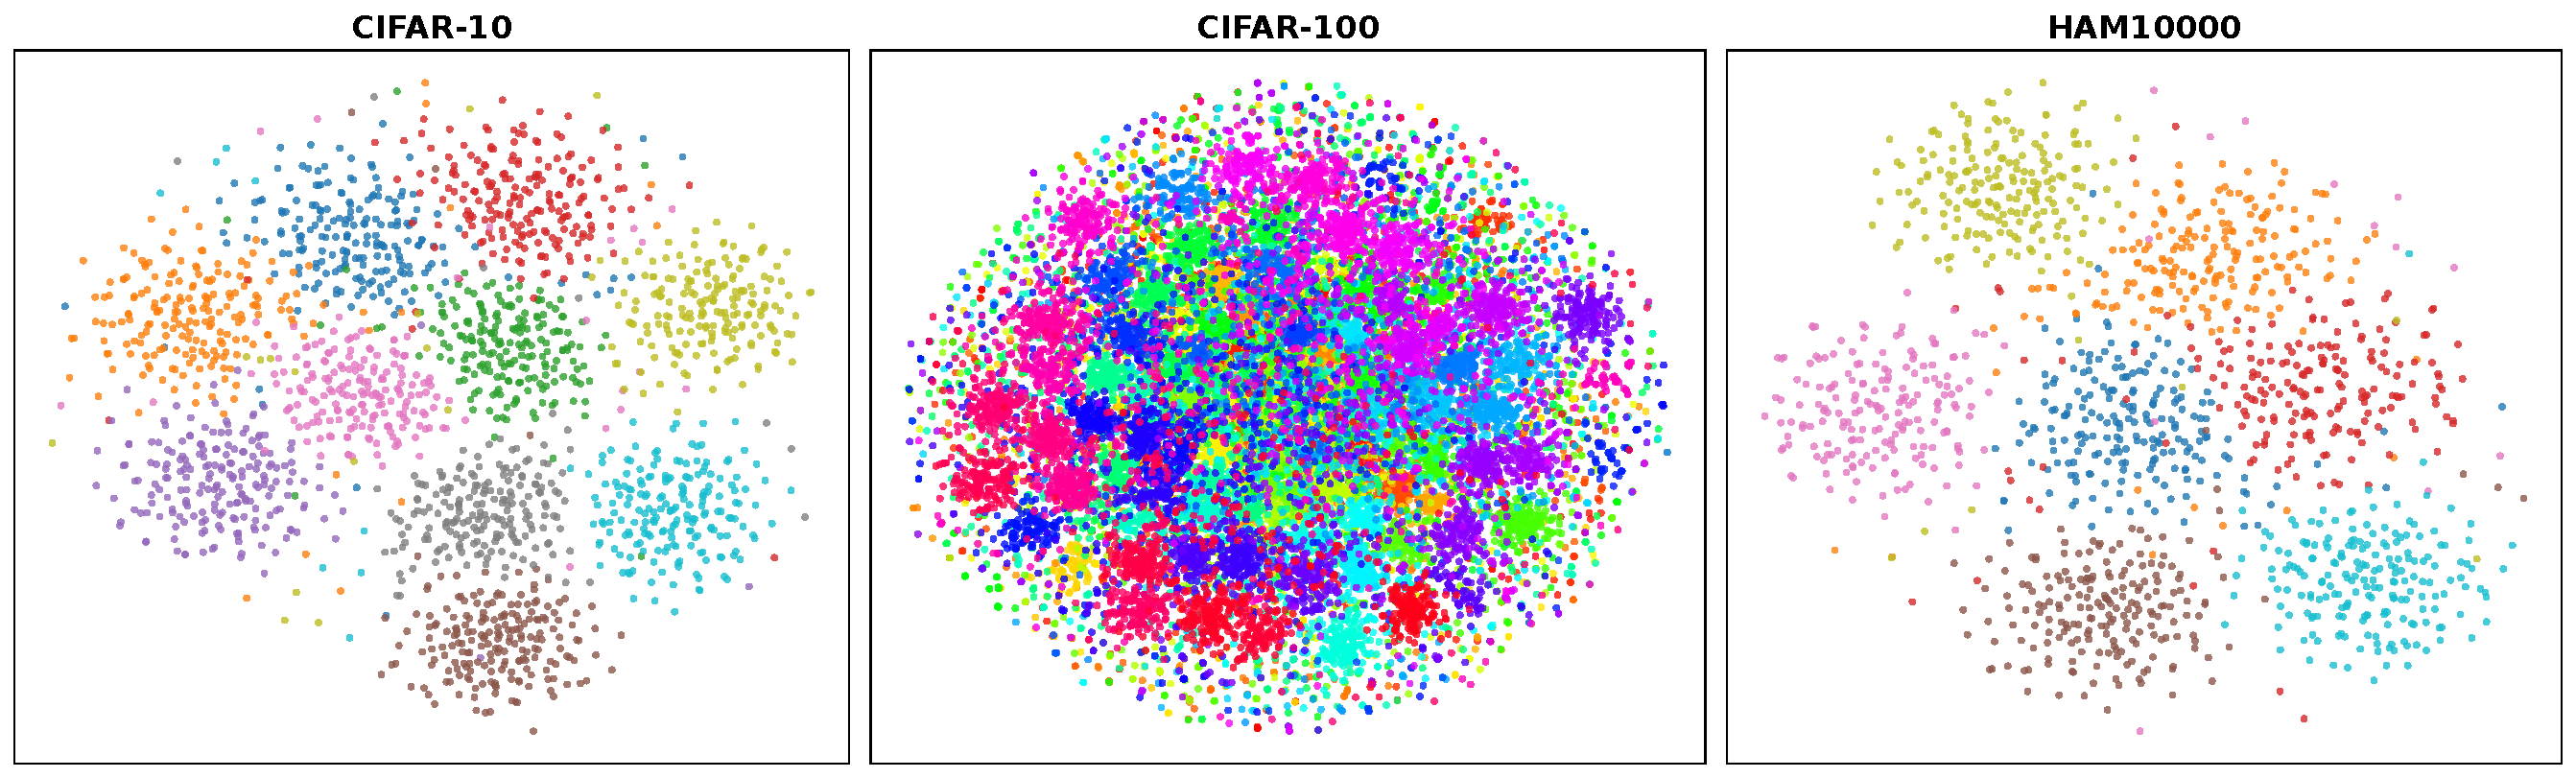
\includegraphics[width=\linewidth]{Figures/tsne_tier2_synthetic.pdf}
        \caption{Refined edge features. Generative aggregation successfully stabilizes distributions, yielding well-separated class clusters.}
        \label{fig:tsne_tier2}
    \end{minipage}
\end{figure}
To qualitatively validate the effectiveness of our multi-tier generative process, we visualize the feature representations at different tiers using T-SNE. \Cref{fig:tsne_tier1} shows the combined feature outputs from clients across all three datasets.  When aggregated from all unaligned clients, they are chaotic and lack any discernible class structure. This offers a challenge of client drift, where each client learns an effective but different local feature space, resulting in an overlapped and nondiscriminative global representation. In contrast, \Cref{fig:tsne_tier2} visualizes the feature space after the edge server's generative aggregation. This visual evidence supports our core claim. Instead of propagating error, the generative aggregation acts as a refinement and stabilization mechanism. It successfully filters the chaotic client-level representations (\Cref{fig:tsne_tier1}) and transforms them into the highly discriminative, globally consistent feature space shown in \Cref{fig:tsne_tier2}.
% \subsection*{Ablation on Temperature Hyperparameter}
% \label{sec:supp_temp_ablation}
% \begin{table}[htbp]
%     \centering
%     \caption{Ablation on the temperature hyperparameter $\tau$ of H-SFP. Results show the Accuracy (\%) at client-edge interval $I_c=5$ and edge-cloud interval $I_e=10$. Results are averaged over 5 independent runs (mean $\pm$ std). The optimal performance is consistently achieved at $\tau=0.5$.}
%     \label{tab:temp_ablation}
%     \resizebox{\textwidth}{!}{
%     \begin{tabular}{l ccc ccc ccc}
%         \toprule
%         \multirow{2}{*}{\textbf{$\tau$}} & 
%         \multicolumn{2}{c}{\textbf{CIFAR-10}} &
%         \multicolumn{2}{c}{\textbf{CIFAR-100}} &
%         \multicolumn{2}{c}{\textbf{HAM10000 (ResNet-50)}} \\ 
%         \cmidrule(lr){2-3} \cmidrule(lr){4-5} \cmidrule(lr){6-7}
%         & \textbf{IID} & \textbf{$dir(0.7)$} & \textbf{IID} & \textbf{$dir(0.7)$} & \textbf{IID} & \textbf{$dir(0.7)$} \\
%         \midrule
%         0.2 & 55.30 {\scriptsize $\pm$ 1.15} & 36.20 {\scriptsize $\pm$ 1.35} & 48.15 {\scriptsize $\pm$ 1.20} & 6.20 {\scriptsize $\pm$ 0.95} & 71.42 {\scriptsize $\pm$ 1.10} & 30.55 {\scriptsize $\pm$ 1.25} \\
%         \textbf{0.5} & \textbf{67.44 {\scriptsize $\pm$ 0.85}} & \textbf{48.85 {\scriptsize $\pm$ 1.10}} & \textbf{55.10 {\scriptsize $\pm$ 0.95}} & \textbf{10.48 {\scriptsize $\pm$ 0.85}} & \textbf{80.86 {\scriptsize $\pm$ 0.75}} & \textbf{37.50 {\scriptsize $\pm$ 1.05}} \\
%         1.0 & 63.15 {\scriptsize $\pm$ 0.95} & 43.10 {\scriptsize $\pm$ 1.20} & 52.88 {\scriptsize $\pm$ 1.05} & 8.50 {\scriptsize $\pm$ 0.90} & 77.40 {\scriptsize $\pm$ 0.90} & 34.70 {\scriptsize $\pm$ 1.15} \\
%         1.5 & 60.03 {\scriptsize $\pm$ 1.05} & 41.50 {\scriptsize $\pm$ 1.25} & 51.10 {\scriptsize $\pm$ 1.10} & 7.20 {\scriptsize $\pm$ 0.95} & 75.85 {\scriptsize $\pm$ 0.95} & 33.10 {\scriptsize $\pm$ 1.20} \\
%         2.0 & 56.38 {\scriptsize $\pm$ 1.10} & 38.40 {\scriptsize $\pm$ 1.30} & 48.65 {\scriptsize $\pm$ 1.15} & 6.05 {\scriptsize $\pm$ 1.00} & 72.12 {\scriptsize $\pm$ 1.05} & 30.45 {\scriptsize $\pm$ 1.25} \\
%         \bottomrule
%     \end{tabular}
%     }
% \end{table}
% \noindent\textbf{Ablation on Temperature $\tau$.}~We investigate the contrastive loss temperature $\tau$ in \Cref{tab:temp_ablation}. The results show a clear ``Goldilocks'' effect. A low $\tau$ (e.g., $0.2$) is too sharp and unstable, while a high $\tau$ (e.g., $2.0$) is too soft and provides an insufficient learning signal. We find $\tau=0.5$ consistently achieves the optimal accuracy across all datasets, balancing feature discrimination and training stability.

